\section{Pain}
Pain is defined, by the International Association for the Study of Pain (IASP), as an unpleasant sensory and emotional experience associated with actual or potential tissue damage \cite{(Marsky and Bogduk, 1994}. Pain is a sudden or slow onset of any intensity from mild to severe pain~\cite{Mello2016} and can categorized based on the pain experience as acute, chronic and intermittent pain~\cite{Goldberg2011}. Acute pain is anticipated or predictable, while  chronic pain is not anticipated or predictable. Chronic pain has a duration greater than three months with a constant or recurring of pain ~\cite{Mello2016}. 

Pain is a worldwide problem and affects all populations regardless of gender, age, income, ethnicity or geography, but the distribution across the globe differs\cite{Goldberg2011}. 
The prevalence and incidence is high despite the complexity of quantifying pain\cite{Goldberg2011}. It is estimated that 20\% of the world's populations adults suffer from pain and each year 10 \% is diagnosed with chronic pain~\cite{Goldberg2011}. 

The frequently causes of pain are operations, cancer, osteoand rheumatoid arthritis, injuries and spinal cord problems~\cite{Goldberg2011}. Furthermore, pain can causes to different sequelae, such as depression, inability to work, limit social relationships and suicidal thoughts\cite{Goldberg2011}. 

People with chronic pain often complain of cognitive problems which interfere with their daily functions~\cite{Geisser2018}. Additionally, it is indicated that among people with chronic pain there is a consistent evidence for disturbances in attentional capacity, processing speed, and psychomotor speed~\cite{Geisser2018}. However, the relationship between pain and cognitive problems is unknown~\cite{Geisser2018}. 

\subsection{Types of pain}
 Pain can be divided into nociceptor pain and neuropathic pain~\cite{Steeds2013}. Nociceptor pain can be classify attending to the location of pain as somatic pain or visceral pain. Somatic pain occurs when nociceptors in skin, muscles, skeleton, joints, or connective tissues are activated. Visceral pain, is defined as pain that results from the activation of nociceptors in the thoracic, pelvic, or abdominal viscera. Unlike somatic pain, visceral pain is harder to localize within the body.  On the other hand, neuropathic pain is caused by a primary lesion or dysfunction of the Peripheral Nervous System (PNS) or Central Nervous System (CNS). The main difference from nociceptor pain is that neuropathic pain has an absence of continuous nociceptive inputs \cite{neuropathic pain}. 
 

 \subsubsection{Nociceptor pain}
Nociceptors are free nerve endings and have a high threshold for mechanical, chemical or thermal stimulation~\cite{Steeds2013}. There are two types of nociceptors $\alpha\delta$ and C fibers. $\alpha\delta$ fibers are very small, between 2-5$\mu$m, myelinated nerve cells, which produce fast well localized sharp pain~\cite{Steeds2013}. The distribution of these fibers are in the body surface, muscles and joints. C fibers are small, <2$\mu$m, unmyelinated nerve cells, and produce slow and poorly localized burning and throbbing pain~\cite{Steeds2013}. The distribution of this fiber type is in most tissues~\cite{Steeds2013}. 
 
When a noxious stimulation occur the nociceptors will be activated and propagate the pain information to the spinal cord nearby via dorsal horn~\cite{Martini2012}.  The second order neuron is activated by the release of nerotrasmitters from the nociceptor. The second order neuron receive these information and cross over to the opposite side of the spinal cord and brings the information towards the brain via the lateral spinothalamic trac. This information will be transmitted by releasing neurotransmitters to the third order neuron in the thalamus. The third order neuron localizes and discriminates the pain in the brain, as illustrated on \figref{fig:somatosensorycortex}, but reverse from where the pain actually had occured. Perception of pain on the right side of the body is processed on the left side of the brain and vice versa~\cite{Martini2012}. 


\begin{figure}[H]
	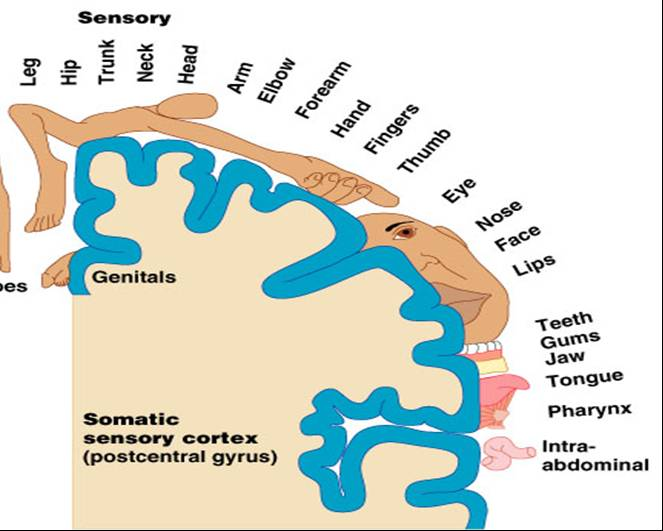
\includegraphics[width=.8\textwidth]{figures/somatosensorycortex.jpg} 
	\caption{Somatosensory cortex .... }
	\label{fig:somatosensorycortex}  
\end{figure}   


\begin{figure}[H]
	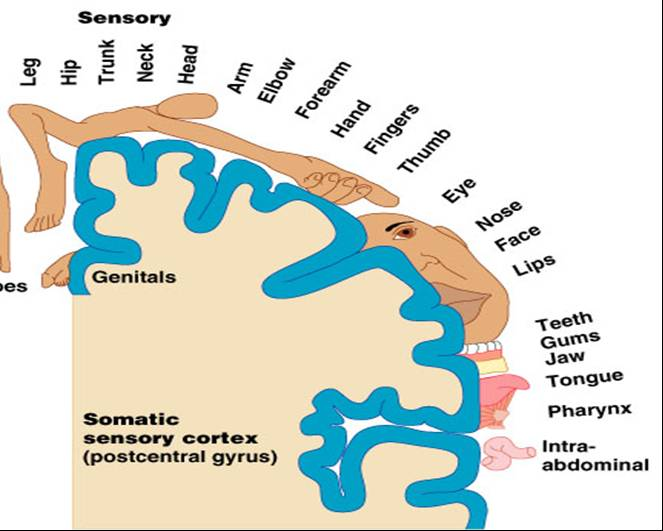
\includegraphics[width=.8\textwidth]{figures/somatosensorycortex.jpg} 
	\caption{Somatosensory cortex .... }
	\label{fig:somatosensorycortex}  
\end{figure}   

Pain is modulated by the descending pathways, where the Periaqueductal Grey (PAG) and the Nucleus Raphe Magnus (NRM) are involved in reducing pain~\cite{Steeds2013}. PAG, also known as anti-nociceptor, is important in the control of pain and surrounds the cerebral aqueduct in Mesencephalon~\cite{Steeds2013}. When this region is electrical stimulated it produces profound analgesia and injection of morphine. PAG receives inputs from the thalamus, hypothalamus, cortex and the spinothalamic tract~\cite{Steeds2013}. Neurons from the PAG region excite the cells in NRM which have a direction towards the spinal cord and block the pain transmission by the dorsal horn cells~\cite{Steeds2013}. Stimulation of NRM produce a strong analgesia and release serotonin which activates the inhibitory interneuron and blocks the pain transmission~\cite{Steeds2013}. The key neurotransmitter is noradrenaline and 5-hydroxytryptamine by modulation pain~\cite{Steeds2013}. 


  \subsubsection{Neuropathic pain}
  
  The most common presentations of this condition are \textit{hyperalgesia}  and \textit{allodynia}. 
  
  
  is often defined as a chronic condition related to the injuries or diseases. Neuropathic pain is caused by a disorder in the somatosensory system~\cite{Mindruta2013}. The disease occurs at different levels in the nervous system and affects the signaling of pain~\cite{Mindruta2013}. The neuropathic pain would not be described as a single cause or a single specific lesson, but instead, they would be described based on a mechanism~\cite{Mindruta2013}. This mechanism can, however, produce painful symptoms in the same disease, by it would take different aspects~\cite{Mindruta2013}.